\begin{appendices}
\chapter{}
\label{chapter:appendix}
\vspace{-20pt}

Here, we present additional material that may answer some questions that the reader might have when reading the main text.

\paragraph{$\ell_{2}$ vs $\ell_{\infty}$ norm}: Why not use $\ell_{2}$ norm instead of $\ell_{\infty}$ norm to report the quantitative results in Figure~\ref{fig:hcp_scatter} or Figure~\ref{fig:dgw_scatter}? The reason is that the $\ell_{2}$ norm will average across the sensors. If one sensor is badly corrupted, then this would not be obvious with the $\ell_{2}$ norm because the average in the $\ell_{2}$ norm computation conceals the isolated problematic sensors with large artifacts. However, as the $\ell_\infty$ norm captures the worst sensor, it can be used to visualize pathological cases where even one sensor is corrupted. In Figure~\ref{fig:l2_norm}, we reproduce Figure~\ref{fig:hcp_scatter} using the $\ell_2$ norm instead of $\ell_{\infty}$. We can observe that, although the pattern remains the same, it is much less clear where one method outperforms the other. Even where \emph{autoreject} isn't performing as well, it is not  visible due to the averaging % effect.

\begin{figure}[htb]
	\centering
	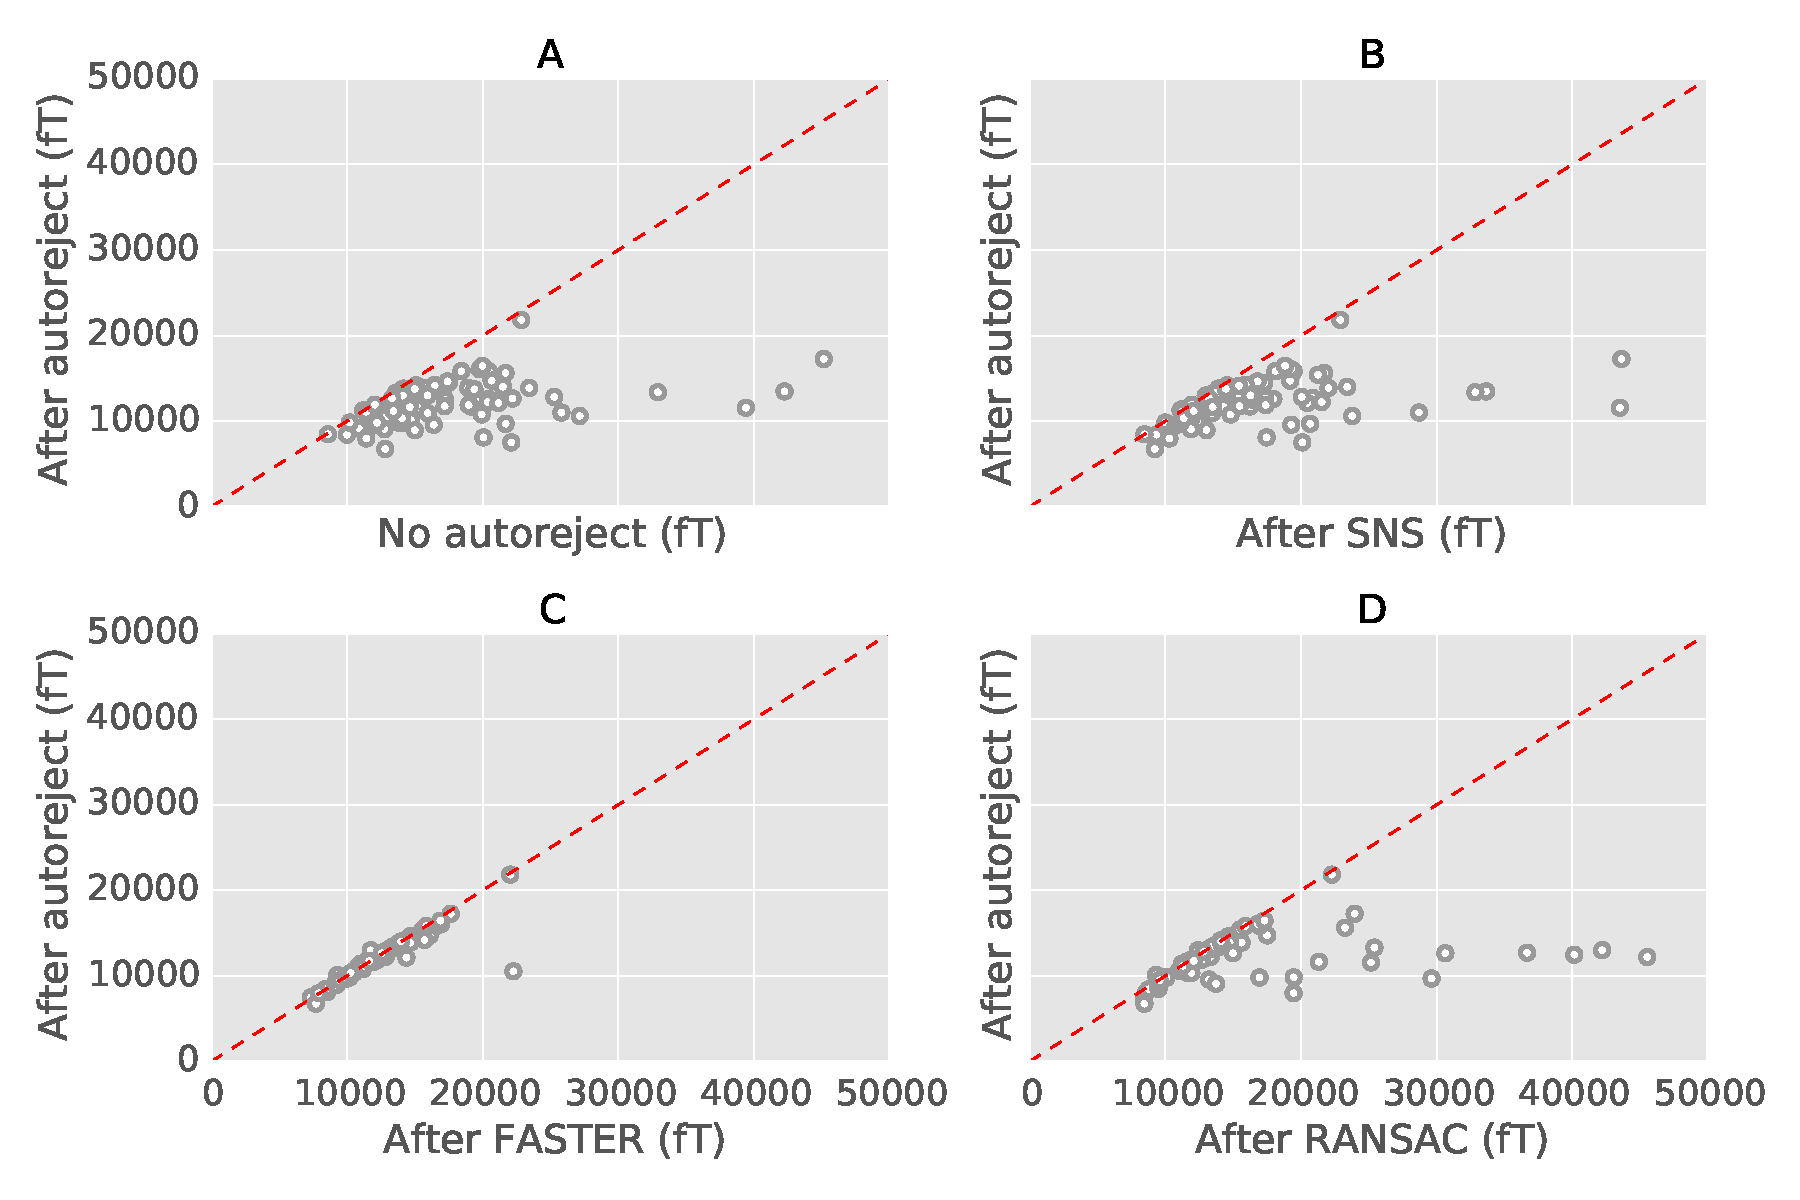
\includegraphics[width=0.8\linewidth]{figures/figure4_supp.pdf}
    \caption[Scatter plots for the results with the HCP data with $l2$ norm instead of $l_\infty$ norm]{Scatter plots for the results with the HCP data. This figure uses the same data as in Figure~\ref{fig:hcp_scatter} from the main text, but with  $\|\cdot\|_2$ norm instead of the $\|\cdot\|_\infty$ norm for computing the difference between the HCP ground truth and the method. As before, each circle is a subject. (A) \textit{autoreject (local)} against no rejection, (B) \textit{autoreject (local)} against Sensor Noise Suppression (SNS) (SNS), (C) \textit{autoreject} against FASTER, (D) \textit{autoreject (local)} against RANSAC. Data points below the dotted red line indicate subjects for which \textit{autoreject (local)} outperforms the alternative method.}
    \label{fig:l2_norm}
\end{figure}

\end{appendices}